\documentclass{article}
\usepackage[utf8]{inputenc}


\title{iacv-project}
\author{shalby.hazem.sh }
\date{August 2022}

\usepackage{graphicx}
\usepackage{multirow}
\usepackage{caption}
\usepackage{subcaption}
\usepackage{tabularx}
\usepackage[backend=biber, style=numeric, sorting=none]{biblatex}
\usepackage{hyperref}
\addbibresource{bibliography.bib}
\graphicspath{ {images} }
%%json
\usepackage[section]{minted} % For code blocks
\newenvironment{code}{\captionsetup{type=listing}}{}
\usepackage[many]{tcolorbox}
\tcbuselibrary{minted}

\newtcbinputlisting{\mycode}[2]{%
  listing engine=minted,
  minted language={#1},
  listing file={#2},
  minted options={
    autogobble=true,
    baselinestretch=1.2,
    fontsize=\footnotesize,
    breaklines=true,
    encoding=utf8
    },
  listing only,
  breakable,
  enhanced jigsaw,
  colframe=black,
  sharp corners,
  boxrule=1pt,
  colback=lightgray!10,
  width=\linewidth
}

%remove red square
\usepackage{etoolbox,xpatch}
\makeatletter
\AtBeginEnvironment{minted}{\dontdofcolorbox}
\def\dontdofcolorbox{\renewcommand\fcolorbox[4][]{##4}}
\xpatchcmd{\inputminted}{\minted@fvset}{\minted@fvset\dontdofcolorbox}{}{}
\xpatchcmd{\mintinline}{\minted@fvset}{\minted@fvset\dontdofcolorbox}{}{} % see https://tex.stackexchange.com/a/401250/
\makeatother

% The following code is only to create the query files
\usepackage{filecontents}
%query1
\begin{filecontents*}{json_example.v}
{
	"barchette": {
		"width": 0.192,
		"height": 0.241,
		"depth": 0.061
	},
	"camomilla": {
		"width": 0.1524,
		"height": 0.0762,
		"depth": 0.0762
	},
	"frontline": {
		"width": 0.14,
		"height": 0.104,
		"depth": 0.012
	},
	"herolight": {
		"width": 0.145,
		"height": 0.142,
		"depth": 0.035
	},
	"infuso": {
		"width": 0.074,
		"height": 0.075,
		"depth": 0.066
	},
	"kellogs_classic": {
		"width": 0.194,
		"height": 0.305, 
		"depth": 0.095 
	},
	"krave": {
		"width": 0.192,
		"height": 0.241, 
		"depth": 0.055
	}
}
\end{filecontents*}


\begin{document}

\begin{titlepage}
	\centering
	\hrule
	\vspace{0,5cm}
	\Huge \textbf{Image Analysis and Computer Vision}
	\vspace{0,5cm}
	\hrule
	\vspace{2,0cm}
	{\Huge \textbf{F10. Template matching in depth images\\}}
		\vspace{0,5cm}
		%\large {Vincenzo Caglioti, Luca Magri, Giacomo Boracchi}
		\vspace{2,5cm}
		{
			\large
			\begin{tabular}{c c}
				Corti Greta & (Personal Code: 10598667)\\
                Chiari Giuseppe & (Personal Code: 10576799) \\
				Shalby Hazem & (Personal Code: 10596243) \\
			\end{tabular}
			
		}
		\vspace{2cm}
		\vspace{0,5cm}
		
		\centering\hspace{0,2cm}
\includegraphics[scale=0.6]{./image/logo.png}
		\vspace{1,5cm}
		
		
		\end{titlepage}

%\tableofcontents

\section{Problem formulation}
Template matching is a very practical technique for finding all the occurrences of a known target in a given query image. Deep-learning techniques are not very flexible, requiring re-training for new templates. Traditional computer vision techniques (e.g. SIFT + RANSAC) are more practical but require an underlying model (homography) describing the transformation between the template and its occurrences in the query image. When there are several occurrences of the same template in the scene, template matching becomes a robust multi-model fitting problem, which requires disambiguating among multiple spurious matches.

The goal of this project is to expand a template detection pipeline based on images only, to RGB-D data. Point clouds should be leveraged to constrain the homography search in regions belonging to the same planar surface in the scene.\\
Another research direction would be to adaptively identify which areas of the target image to search, which is a very relevant problem when the number of key points is large (e.g. a few hundred) by exploiting the 3D data of the scene.

The specific case tackled by the following project is recognizing squared boxes in the scene, such as those found in a supermarket.

\begin{figure}[H]
    \centering
     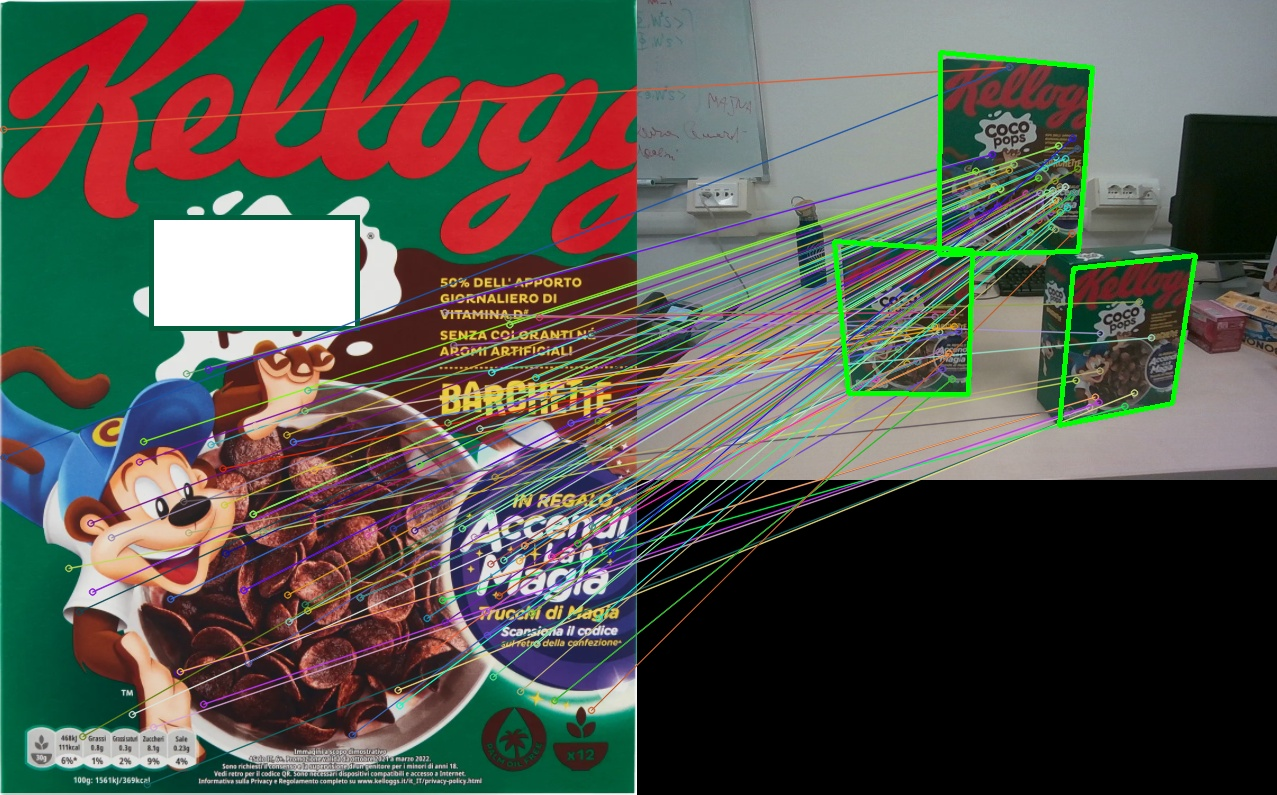
\includegraphics[width=\textwidth]{image/matching_example.jpg}
    \caption{Template Matching example}
\end{figure}

\section{State of the art} %greta 
% Riscrivere paragrafo come gli altri ragazzi ma con parole nostre. Citare SIFT e ORB, dicendo due parole su pro e contro dei due metodi. Breve spiegazione della pipeline del template matching.
The Template Matching method simply scans the complete image and slides over the template image across the full image and identifies the matching area as a heatmap: this method is mostly static and it gives very poor results if the full image has slight deviations like the direction change, image intensity change, scale changes. Hence, it cannot be used in real-world applications. \\

\begin{figure}[H]
    \centering
     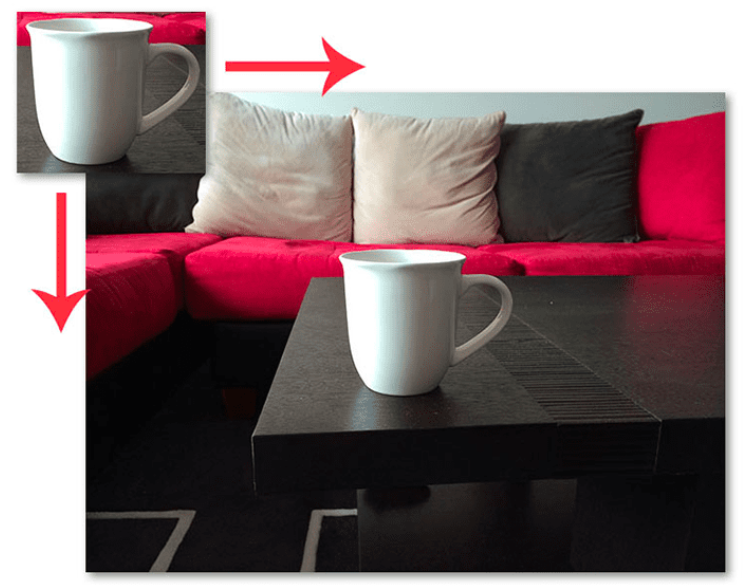
\includegraphics[width=0.5\textwidth]{image/template_matching_sliding.png}
    \caption{The easiest way to do template matching}
\end{figure}

To overcome the above difficulties of the Template Matching method, key point detectors are the solution. Key points may be defined as small areas of an image having some particular features, e.g. rapid changes in image brightness domain, like corners. A set of detected key points and parameters describing them, known as descriptors, collect the most important features of an object and create its representation in a compact structure of a template. In literature, different feature detectors exist: Scale Invariant Feature Transform (SIFT), Speed Up Robust Feature (SURF), and Oriented FAST and Rotated BRIEF (ORB).
SIFT is mainly used because it performs the best in most scenarios and the key point detectors are distributed over the image. ORB is the fastest algorithm, but the extracted features are mostly concentrated in objects at the center of the image. ORB and SURF outperform SIFT only when the angle of rotation is proportional to 90 degrees \cite{karami_prasad_shehata_2017}.\\

Once the features get detected and matched, only 4 matches would be enough to fit the 2D homography mapping the template to the scene's plane, but the reality is that, in any real-world case, several bad matches will occur. After a coarse cleaning of the outliers with a ratio test, an outlier detection method is still needed. In computer vision, random sample consensus (RANSAC) is used as a robust procedure to estimate the foundational matrix in stereo vision, to find if two sets of points are equal. It is a recursive method for estimating a mathematical representation from a data set that contains outliers. The RANSAC algorithm works by identifying the outsiders in a data set and approximating the wanted model using data that does not contain outliers.
Given a set of features F, RANSAC algorithm works as follows:
\begin{enumerate}
  \item Randomly selects a subset S of the original data set F.
  \item Fit a model \textit{M} to the points of S.
  \item All the data belonging to the set F-S are then tested against \textit{M}. Those points that fit \textit{M} well, according to some loss function, are considered as part of the consensus set S. The estimated model \textit{M} is reasonably good if sufficiently many points have been classified as part of S.
  \item Afterwards, the model may be improved by re-estimating it using all members of the consensus set.
  \item Repeat steps 1-4 for a fixed number of iterations.
\end{enumerate}
At each iteration, it will be produced either a model which is rejected because not enough points are part of the consensus set, or a processed model together with a corresponding consensus set size.

\begin{figure}[H]
    \centering
     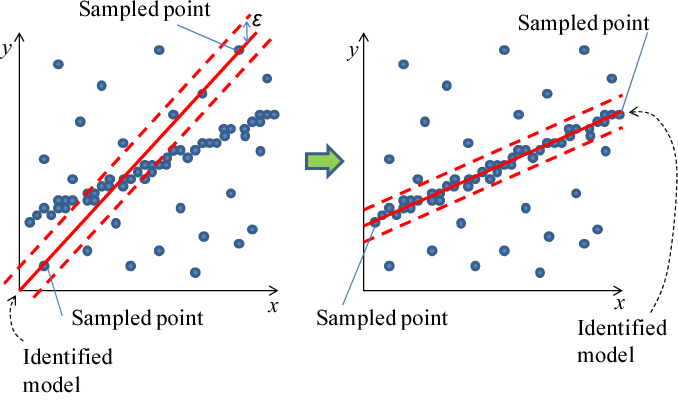
\includegraphics[width=0.5\textwidth]{image/Ransac.png}
    \caption{Conceptual figure of RANSAC}
\end{figure}


\section{Solution approach} %shalby
The most known algorithms that solve the template matching problem, reach the goal by performing the following operations:
\begin{itemize}
    \item feature extraction from the template and the scene.
    \item feature matching and selection.
    \item fit the homographies via sequential Ransac.
\end{itemize}
As can be easily noticed, the most vulnerable parts of the above pipeline are clearly the elaboration of the huge number of features extracted from the scene at the beginning of the process and the identification of key points to use for the computation of the homography.

The approach followed during the project development \cite{corti_chiari_shalby_2022} was to start from the above pipeline and try to improve its performance by acting on the most vulnerable parts; in particular, the techniques implemented use filters to reduce the number of key points to examine and to select the few key points needed to fit the homography in different ways than the ones proposed by Polidori and Stagnoli \cite{polidori_stagnoli_2022}.

In the following sections, three main techniques will be described in detail.

%Filtro
%CustomRansac estrazione casuale
%CustomRansac con rettangoli

%\section{Implementation}
%Intro
%Scrivere come si è implementato ogni metodo

\subsection{Canny Filter Method}
\label{canny_filter}
%Filtro --> greta
To decrease the number of key points extracted by SIFT from the image, a Canny edge detection has been implemented. It is assumed that object edges can be exploited to choose the most useful key points to improve the performance of key point detection and matching \cite{matusiak_skulimowski_strumillo_2018}.
On both RGB scene image and depth image a denoised function is applied a and then the Canny method. On the resulting images, Probabilistic Hough Line Transform is applied; it is more efficient implementation of the Hough Line Transform because it gives as output the extremes of the detected lines. The extracted lines from RGB image are compared with the extracted lines from the depth image so to have more accuracy and precision in line selection since some are wrong due to image noise. Thanks to these lines, probable rectangles can be created and they represent the boxes present on the scene. Having the rectangles and the key points of the scene, all the key points that are outside the rectangles can be deleted. In this way, the number of key points usually decreases by one-third of the initial total number.

\begin{figure}[H]
    \begin{subfigure}[b]{0.5\textwidth}
        \centering
        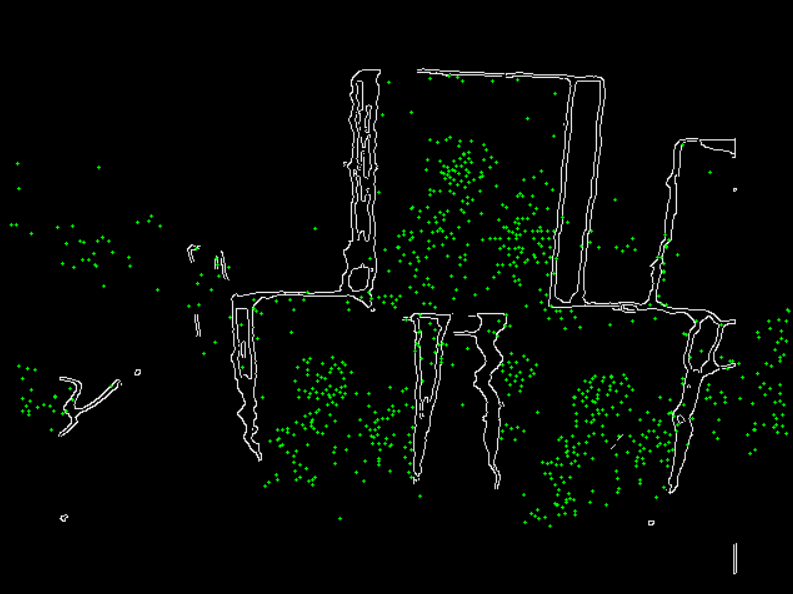
\includegraphics[width=0.8\textwidth]{image/allKeypointsSIFT.png}
        \caption{Key points found by SIFT}
    \end{subfigure}
    \begin{subfigure}[b]{0.5\textwidth}
        \centering
        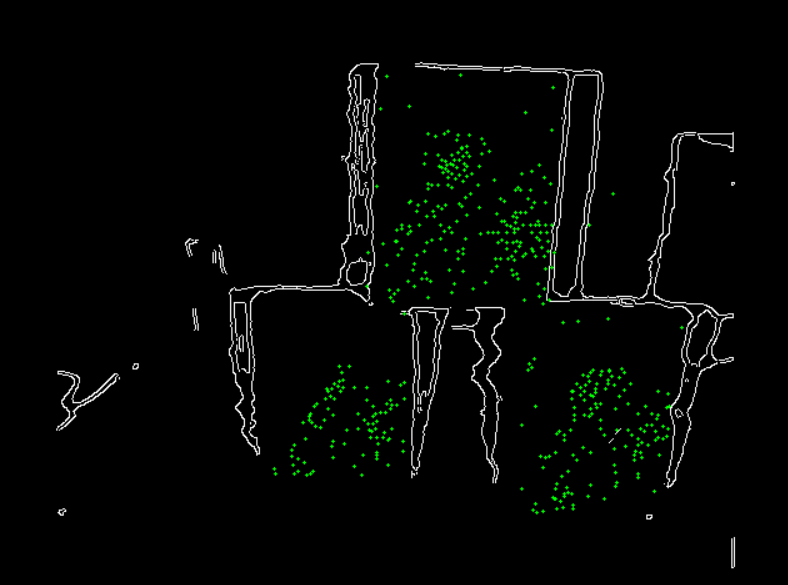
\includegraphics[width=0.8\textwidth]{image/KeypointsByRectangles.png}
        \caption{Key points after applying the filter}
    \end{subfigure}
    \caption{Example of key points found on image 5}
    
\end{figure}

\subsection{Homography based on boxes dimensions}
%CustomRansac estrazione casuale --> giuseppe
This technique is based on randomly extracting one key point and then finding other three key points around it, so to be able to find an homography with four key points.

The last three key points are to be found near the first one, where \textit{near} is specified by the template's dimensions: each template is defined by a \textit{width}, \textit{height} and \textit{depth}, expressed in centimeters (see below). The coordinates of the last three key points should be no further away from those of the first one than the dimensions found in the \textit{dimensions.json} file, depending on the template.

Clearly, the approach has to be carried out after key points identification: a task that can be completed either with or without the use of \nameref{canny_filter}. The use of the filter can influence execution time and consistency, as illustrated in \nameref{results}.

The main flaw of this approach is its dependence on randomization, which is key in improving performance, but it can also lead to slightly different solutions each time the algorithm is run.\\


\begin{code}
    \mycode{json}{json_example.v}
    \caption{JSON file containing boxes dimensions}
\end{code}

\subsection{Homography based on Rectangles}
The proposed approach is based on the identification of Rectangles inside the scene and then uses them to select the regions of the image in which the algorithm can match the template. 
In particular, the whole process can be divided into the following steps:
\begin{enumerate}
    \item Identify the rectangles inside the scene;
    \item Filter the key points by keeping the ones that are inside at least one of the identified rectangles; 
    \item Iterate over the rectangles and run Ransac as follows:
    \begin{enumerate}
        \item select randomly four points from the ones inside the considered rectangle
        \item Use the selected points to compute the Homography
    \end{enumerate}   
\end{enumerate}

The use of rectangles to identify the area to analyze is due to the geometry of the boxes (template) to identify.\\

%The identification of the areas in which the algorithm is more probable to match the pattern can be also seen as a filtering approach in which only the key points inside rectangles are used in the rest of the process. In the proposed implementation, rectangles are used both to filter the key points and to fit the homography.\\

A noteworthy part of this approach is the identification process of rectangles, which is performed by executing the following operations:
\begin{itemize}
    \item Identify lines (Canny $+$ Hough) both from the scene and the Depth Map\footnote{Denoising process of the image and of the Depth Map is performed in order to improve the identification of the lines}
    \item Select the most promising lines
    \item Use pairs of almost perpendicular lines (angle of 70/90 degrees) to identify the rectangles
\end{itemize}

The bottleneck of the whole process is the identification of the rectangles and further improvement of this approach can focus on it.
\begin{figure}[H]
    \begin{subfigure}[b]{0.5\textwidth}
        \centering
        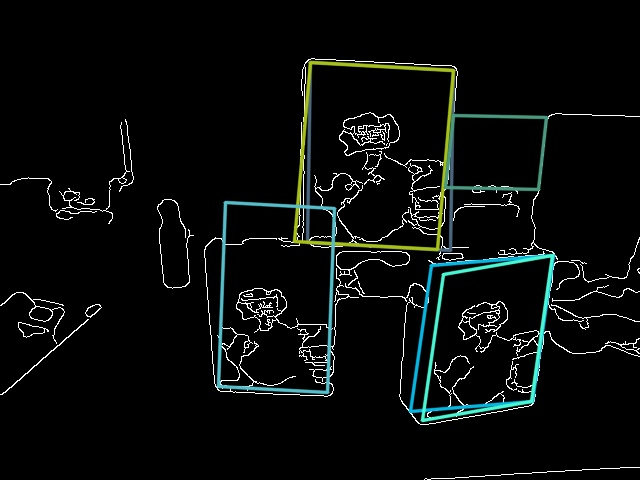
\includegraphics[width=0.8\textwidth]{image/rectangles-example.jpg}
        \caption{identified rectangles}
    \end{subfigure}
    \begin{subfigure}[b]{0.5\textwidth}
        \centering
        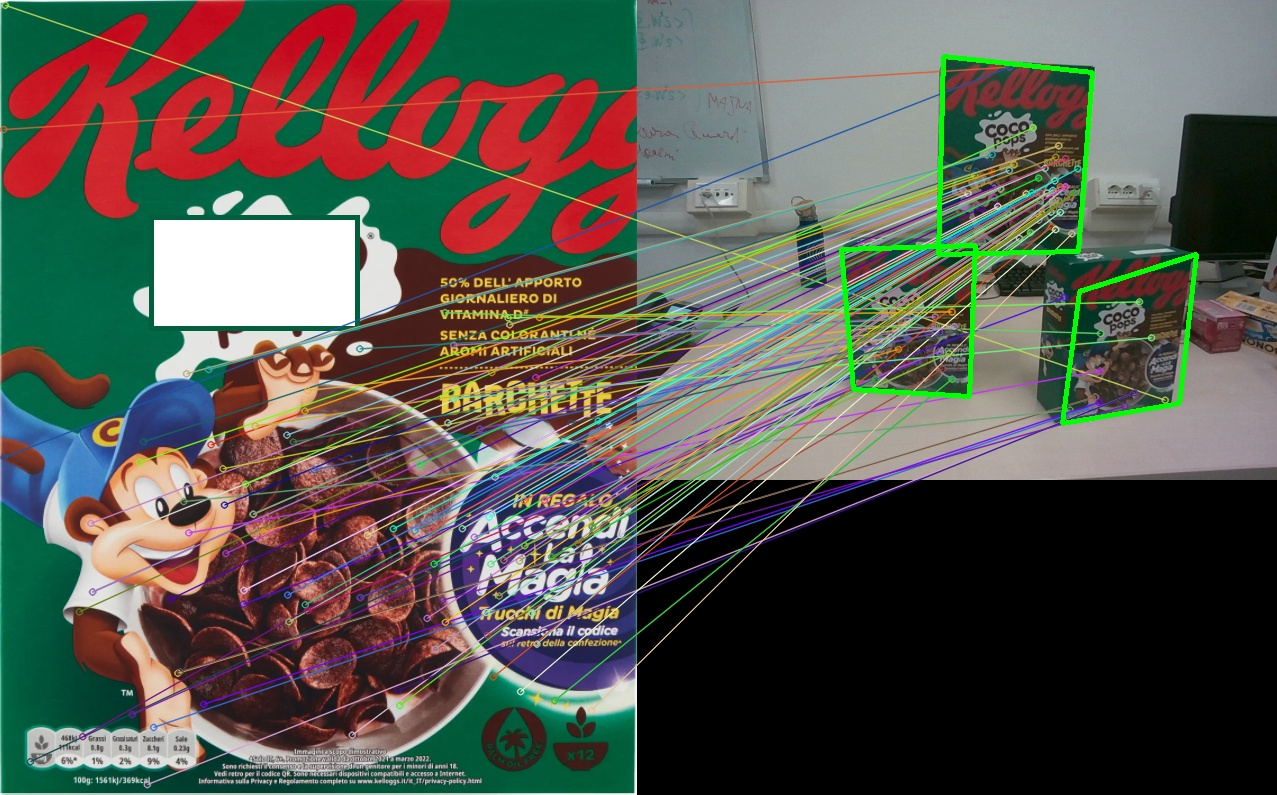
\includegraphics[width=\textwidth]{image/barchette_5_rettangoli.jpg}
        \caption{final results}
    \end{subfigure}
    \caption{Example of rectangles identified on the image 5}
    
\end{figure}


\section{Results} %giuseppe
\label{results}
% Screen di alcune immagine finali con le box.
% Tabelle con i benchmark che mettono a confronto:
% - nostri risultati
% - quelli degli altri ragazzi
% - quelli base
In general, the performance of this type of algorithm is measured in terms of speed; thus, the time of execution is taken as the main index of comparison between the base algorithm and those proposed.

The following results show execution time based on the search of Kellog's Barchette and compare our solutions with those of customFindHomography3D-Plane, developed by Alessandro Polidori and Nicolò Stagnoli \cite{polidori_stagnoli_2022}.

Time is expressed in seconds and has been approximated to the second decimal digit.\\

\begin{figure}[H]
    \centering
    \begin{tabularx}{\textwidth}{||X X X X X||} 
        \hline
     n° box & Dimension w/ filter & Dimension w/o filter & Rectangles & base \\ [0.5ex]
     \hline\hline
     1 & 3.15 & 3.07 & - & 5.94 \\ 
     \hline
     2 & 5.23 & 5.19 & - & 18.58 \\
     \hline
     3 & 6.96 & 6.96 & - & 25.59 \\
     \hline
    \end{tabularx}
    \caption{Image 1}
    \label{imag1}
\end{figure}

\begin{figure}[H]
    \centering
   \begin{tabularx}{\textwidth}{||X X X X X||} 
        \hline
     n° box & Dimension w/ filter & Dimension w/o filter & Rectangles & base \\ [0.5ex]
     \hline\hline
     1 & 2.70 & 2.63 & 0.28 & 5.94 \\ 
     \hline
     2 & 4.79 & 4.83 & 0.47 & 10.72 \\
     \hline
     3 & 6.36 & 6.70 & - & 14.56 \\
     \hline
    \end{tabularx}
     \caption{Image 2}
\end{figure}

\begin{figure}[H]
    \centering
  \begin{tabularx}{\textwidth}{||X X X X X||} 
        \hline
     n° box & Dimension w/ filter & Dimension w/o filter & Rectangles & base \\ [0.5ex]
     \hline\hline
     1 & 2.48 & 2.09 & - & 6.76 \\ 
     \hline
     2 & 4.04 & 3.36 & - & 11.86 \\
     \hline
    \end{tabularx}
     \caption{Image 3}
\end{figure}


\begin{figure}[H]
    \centering
    \begin{tabularx}{\textwidth}{||X X X X X||} 
        \hline
     n° box & Dimension w/ filter & Dimension w/o filter & Rectangles & base \\ [0.5ex]
     \hline\hline
     1 & 2.97 & 2.68 & 0.47 & 6.73 \\ 
     \hline
     2 & 4.48 & 4.15 & - & 12.02 \\
     \hline
    \end{tabularx}
     \caption{Image 4}
\end{figure}

\begin{figure}[H]
    \centering
   \begin{tabularx}{\textwidth}{||X X X X X||} 
        \hline
     n° box & Dimension w/ filter & Dimension w/o filter & Rectangles & base \\ [0.5ex]
     \hline\hline
     1 & 3.75 & 3.84 & 0.53 & 0.07 \\ 
     \hline
     2 & 5.58 & 5.79 & 0.78 & 5.93 \\
     \hline
     3 & 6.89 & 7.01 & 0.92 & 18.29 \\
     \hline
    \end{tabularx}
     \caption{Image 5}
\end{figure}

\begin{figure}[H]
    \centering
   \begin{tabularx}{\textwidth}{||X X X X X||} 
        \hline
     n° box & Dimension w/ filter & Dimension w/o filter & Rectangles & base \\ [0.5ex]
     \hline\hline
     1 & 3.72 & 3.66 & 0.52 & 9.61 \\ 
     \hline
     2 & 5.83 & 5.84 & 0.88 & 14.26 \\
     \hline
     3 & - & - & 1.06 & 18.06 \\
     \hline
    \end{tabularx}
     \caption{Image 6}
\end{figure}

\begin{figure}[H]
    \centering
    \begin{tabularx}{\textwidth}{||X X X X X||} 
        \hline
     n° box & Dimension w/ filter & Dimension w/o filter & Rectangles & base \\ [0.5ex]
     \hline\hline
     1 & 4.40 & 4.20 & 1.58 & 1.23 \\ 
     \hline
     2 & 6.21 & 6.25 & - & 4.11 \\
     \hline
    \end{tabularx}
     \caption{Image avanti\_dietro}
\end{figure}

\begin{figure}[H]
    \centering
   \begin{tabularx}{\textwidth}{||X X X X X||} 
        \hline
     n° box & Dimension w/ filter & Dimension w/o filter & Rectangles & base \\ [0.5ex]
     \hline\hline
     1 & 3.73 & 3.63 & 0.58 & 0.93 \\ 
     \hline
     2 & 5.99 & 5.82 & - & 5.04 \\
     \hline
     3 & 7.65 & - & - & 9.04 \\
     \hline
    \end{tabularx}
     \caption{Image avanti\_dietro2}
\end{figure}

As it can be noted from the tables, all three methods are often faster than customFindHomography3DPlane. In particular, if customFindHomographyRectangles finds rectangles in the image, it can outperform drastically the other methods while maintaining the same precision, as can be seen in the following screenshots.
On the other hand, customFindHomographyDimension (with or without filter) is more consistent, meaning that it finds almost always all the boxes, but it is slower.

\begin{figure}[H]
     \centering
     \begin{subfigure}[b]{0.3\textwidth}
         \centering
         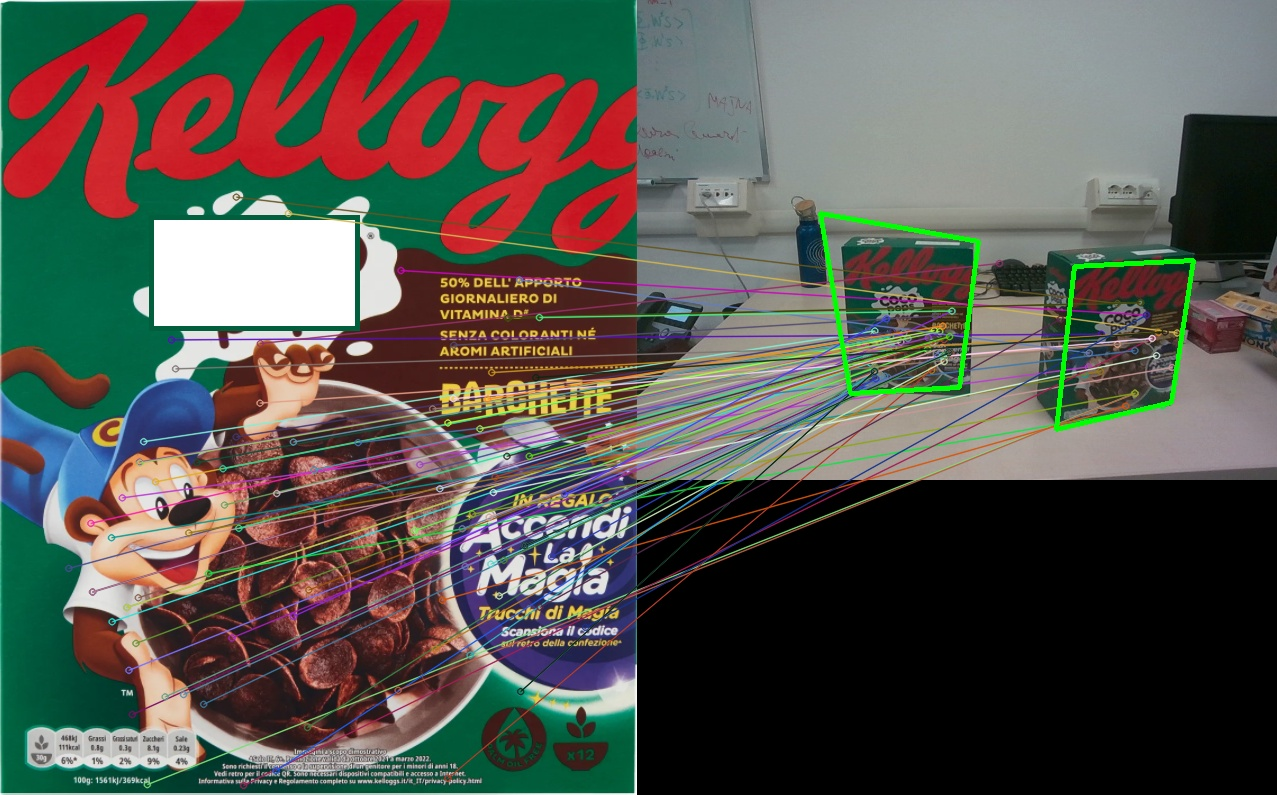
\includegraphics[width=\textwidth]{image/barchette_4_con_filtro.jpg}
         \caption{customFindHomographyDimension with filter}
         \label{fig:customFindHomographyDimension with filter}
     \end{subfigure}
     \hfill
     \begin{subfigure}[b]{0.3\textwidth}
         \centering
         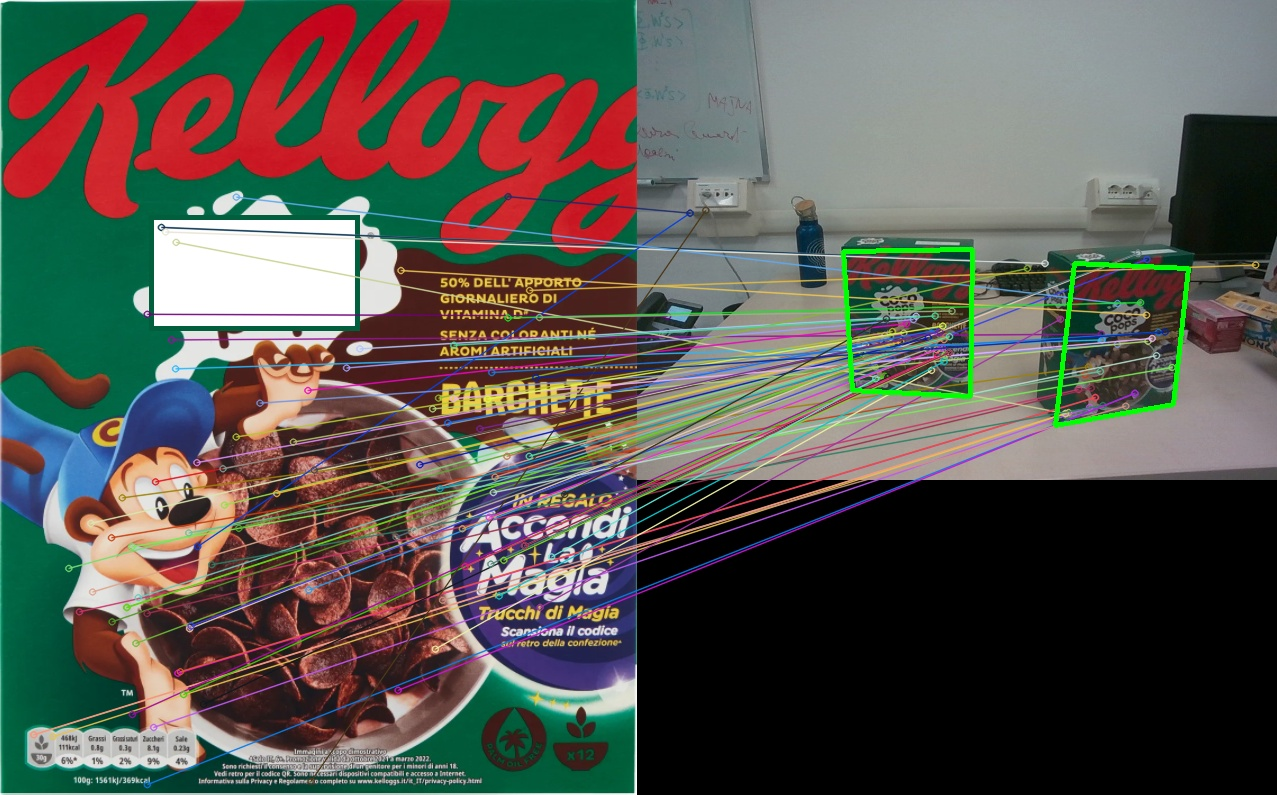
\includegraphics[width=\textwidth]{image/barchette_4_senza_filtro.jpg}
         \caption{customFindHomographyDimension w/o filter}
         \label{fig:customFindHomographyDimension without filter}
     \end{subfigure}
     \hfill
     \begin{subfigure}[b]{0.3\textwidth}
         \centering
         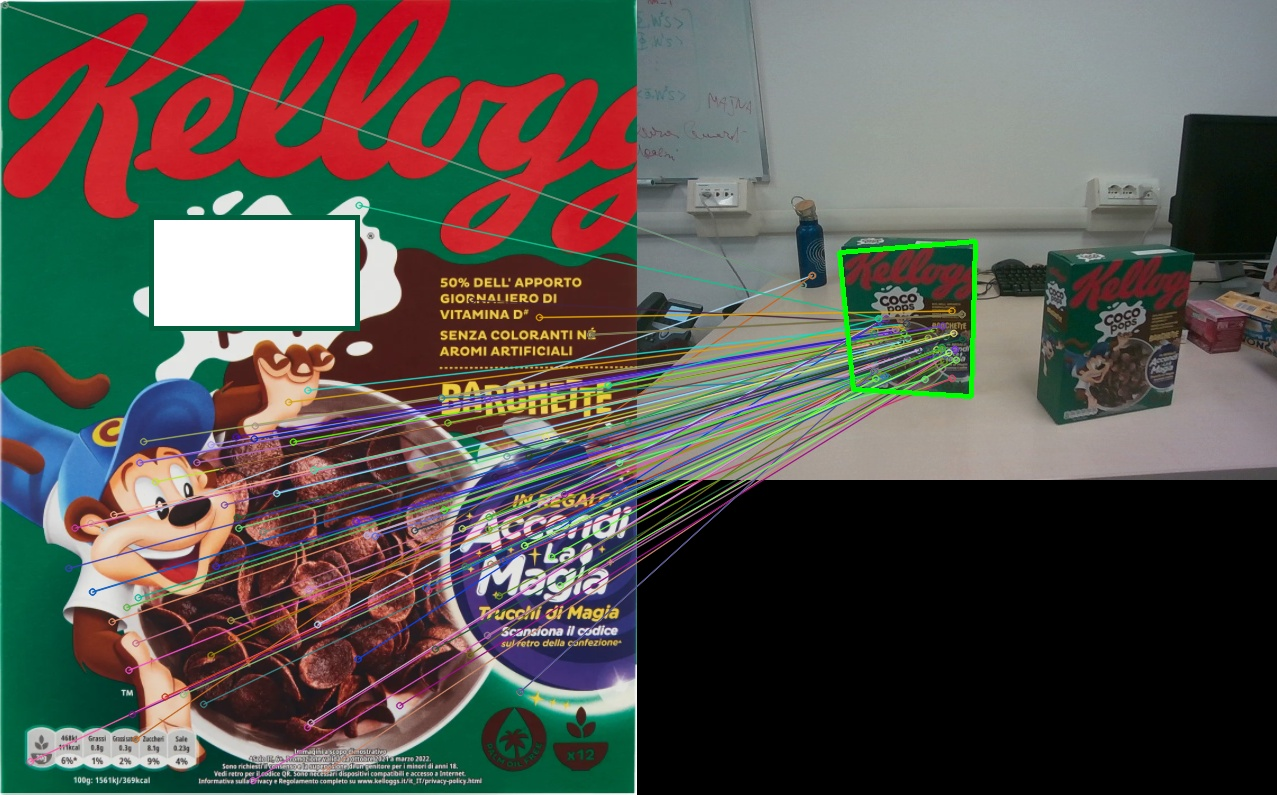
\includegraphics[width=\textwidth]{image/barchette_4_rettangoli.jpg}
         \caption{customFindHomographyRectangles}
         \label{fig:customFindHomographyRectangles}
     \end{subfigure}
     \hfill
        \caption{Image 4}
        \label{fig:image 4}
\end{figure}

\begin{figure}[H]
     \centering
     \begin{subfigure}[b]{0.3\textwidth}
         \centering
         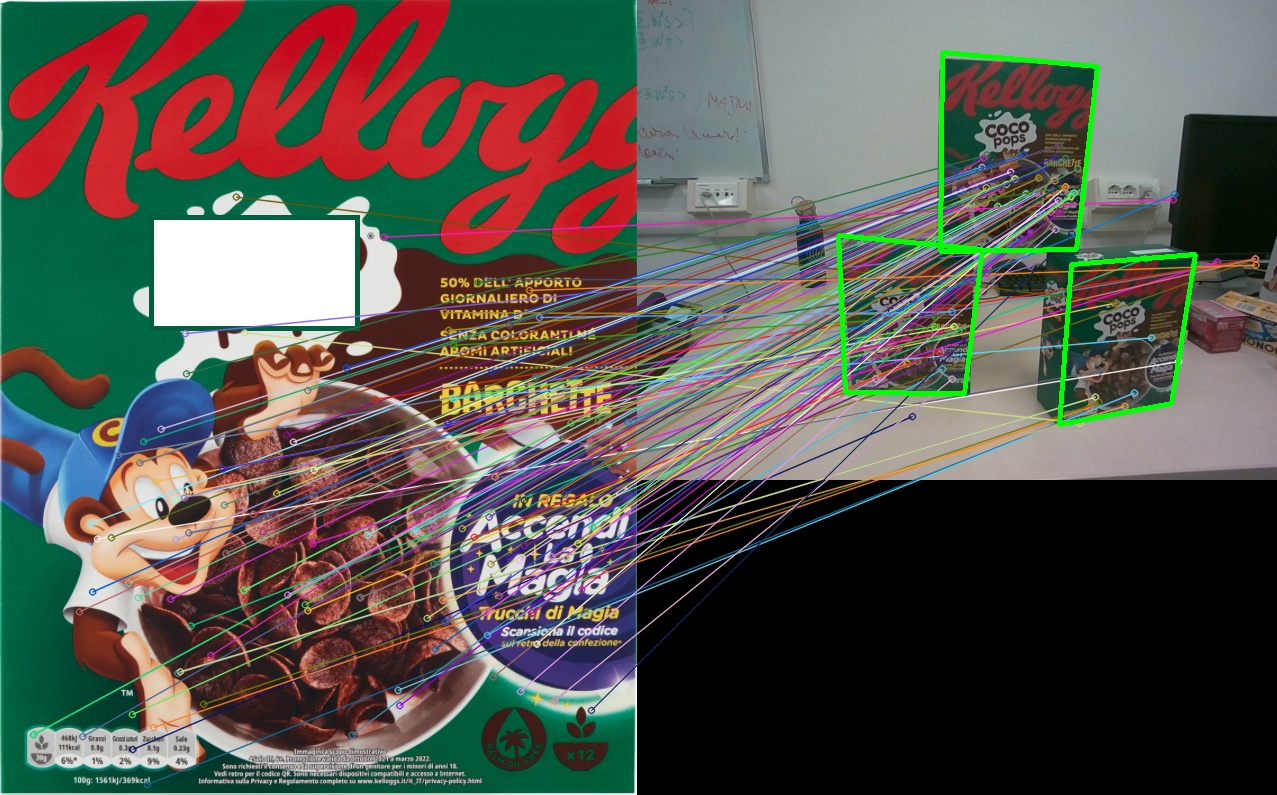
\includegraphics[width=\textwidth]{image/barchette_5_con_filtro.jpg}
         \caption{customFindHomographyDimension with filter}
         \label{fig:customFindHomographyDimension with filter}
     \end{subfigure}
     \hfill
     \begin{subfigure}[b]{0.3\textwidth}
         \centering
         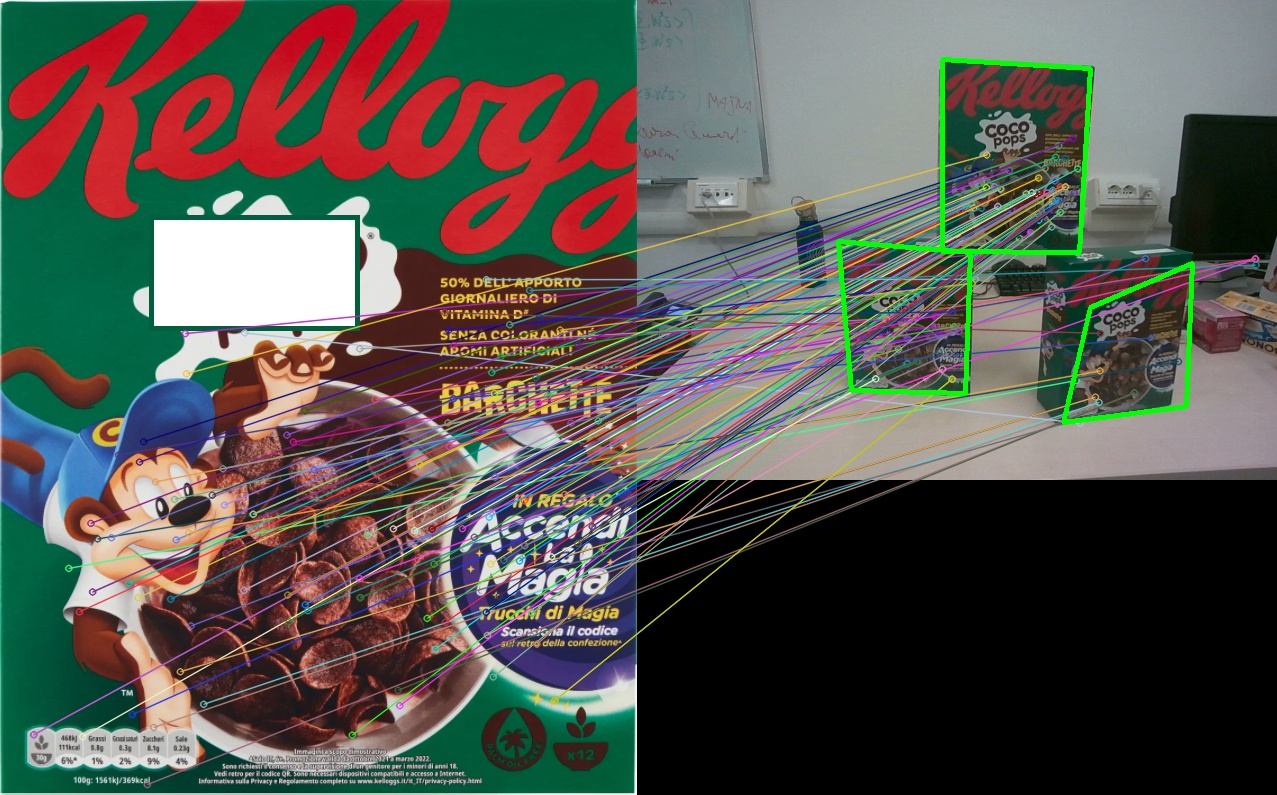
\includegraphics[width=\textwidth]{image/barchette_5_senza_filtro.jpg}
         \caption{customFindHomographyDimension w/o filter}
         \label{fig:customFindHomographyDimension without filter}
     \end{subfigure}
     \hfill
     \begin{subfigure}[b]{0.3\textwidth}
         \centering
         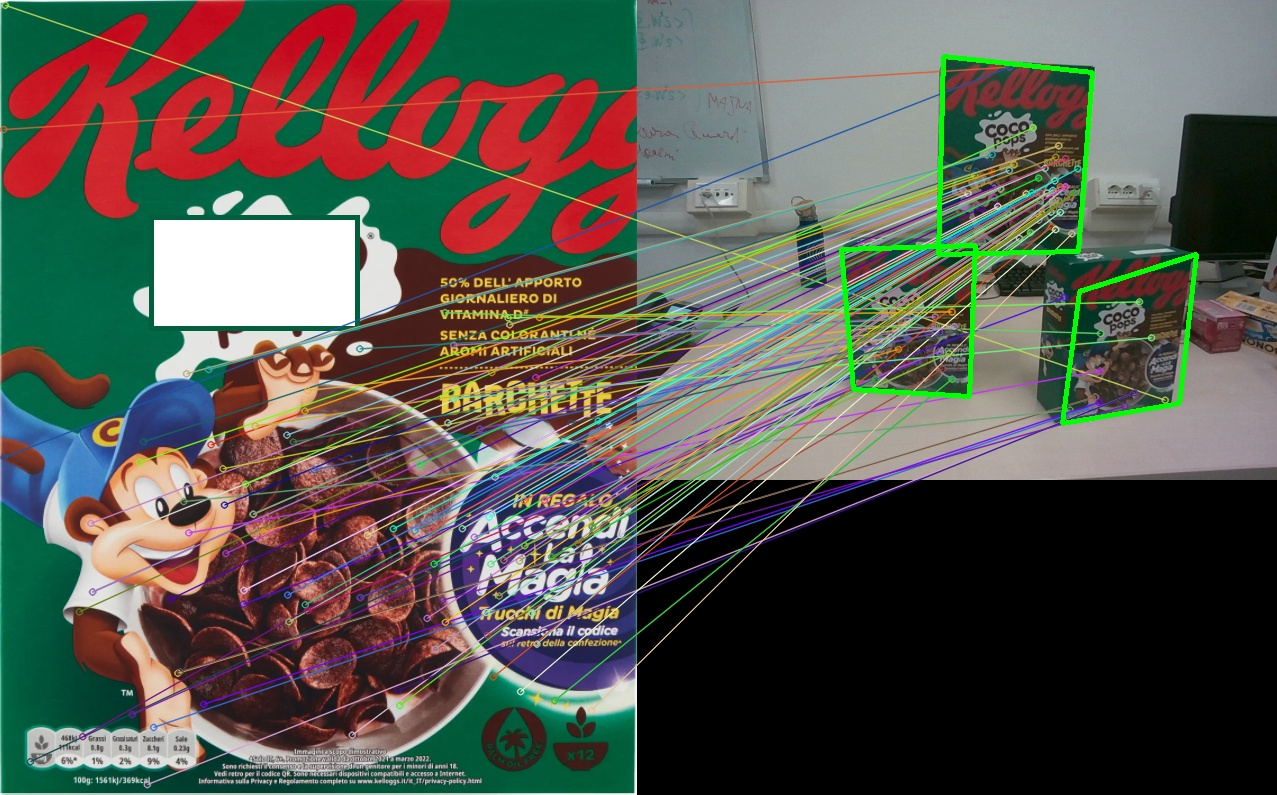
\includegraphics[width=\textwidth]{image/barchette_5_rettangoli.jpg}
         \caption{customFindHomographyRectangles}
         \label{fig:customFindHomographyRectangles}
     \end{subfigure}
     \hfill
        \caption{Image 5}
        \label{fig:image 5}
\end{figure}

\section{Conclusion and open problems}
%Che tipo di miglioramenti ci sono stati con le nostre aggiunte rispetto a quelle degli altri ragazzi
%Problemi trovati ma non stati risolti, magari con possibile soluzione
The report illustrates different techniques to tackle the problem of template matching boxes. Each technique shows different strengths as seen in the above results. Overall there is an improvement in the matter of execution times with respect to the work done by Polidori and Stagnoli \cite{polidori_stagnoli_2022}.

Several issues are left open, such as improving the effectiveness of the rectangles identification in customFindHomographyRectangles.

Another problem is that it may happen that any of the proposed algorithms finds degenerate bounding boxes, which are clearly not linked to any box and have to be removed.

At last, randomization poses a question: different executions of the program may lead to different solutions. While it is key to improving the performance of the proposed algorithms, its impact has to be constrained so not to damage the overall consistency of the program.\\
\\
%%%%% REFERENCES %%%%%
% ad esempio link alla repo github
% e altro...
\printbibliography


\end{document}
